\subsection{Makrozyklus Schritt 2: Entscheidungsfindung durch den Actor}

Nachdem der initiale Schaltungszustand durch eine Zufallsverteilung generiert wurde, kommt der Actor ins Spiel, der auf Basis der aktuellen Kapazitäts- (C) und Induktivitätswerte (L) Entscheidungen trifft. Der Actor, ein wesentlicher Bestandteil des Reinforcement Learning Systems, ist eine komplexe Funktion, die sich aus mehreren Gewichtungen (weights) und Verzerrungen (biases) zusammensetzt. Diese werden im Laufe des Vorwärtsdurchlaufs (Forward Propagation \ref{sec: Forward Propagation}) durch das Netzwerk multipliziert und summiert.

\begin{itemize}
		\item Innerhalb des Actors wird die Eingabe durch jede Schicht des neuronalen Netzwerks transformiert, wobei nach jedem Schichtdurchgang eine nicht-lineare Aktivierungsfunktion \ref{eq:activation_function} angewandt wird, um die Linearität der Operationen zu durchbrechen.
		\item Im spezifischen Kontext unseres Systems ist die Aktivierungsfunktion der letzten Schicht eine  Hyperbelfunktion (tanh), die die Ausgabe des Netzwerks beeinflusst und zu einem komplexen, nicht-linearen Ergebnis führt.
\end{itemize}

Die Ausgabe des Actors sind die PID-Werte, die für die Steuerung des nächsten Schrittes im System verwendet werden. Diese Werte sind das Resultat des durch die tanh-Funktion modifizierten Outputs und stellen somit eine fein abgestimmte Reaktion auf den Zustand der Schaltung dar. Diese Werte werden anschließend skaliert, um realistische PID-Reglerparameter zu erhalten:

\begin{itemize}
	\item Der Proportionalwert (Kp) wird zwischen 0 und 10 skaliert.
	\item Der Integralwert (Ki) wird zwischen 0 und 1 skaliert.
	\item Der Differentialwert (Kd) wird zwischen 0 und 0.1 skaliert.
\end{itemize}

Diese Skalierung ist entscheidend, um die Ausgangswerte des neuronalen Netzes in praktikable Steuerparameter zu überführen. Die Transformation gewährleistet, dass die PID-Werte in einem Bereich liegen, der für die Regelung des Systems adäquat ist und reflektiert die praktischen Anforderungen an die Systemsteuerung. 


\begin{figure}[htbp]
\centering
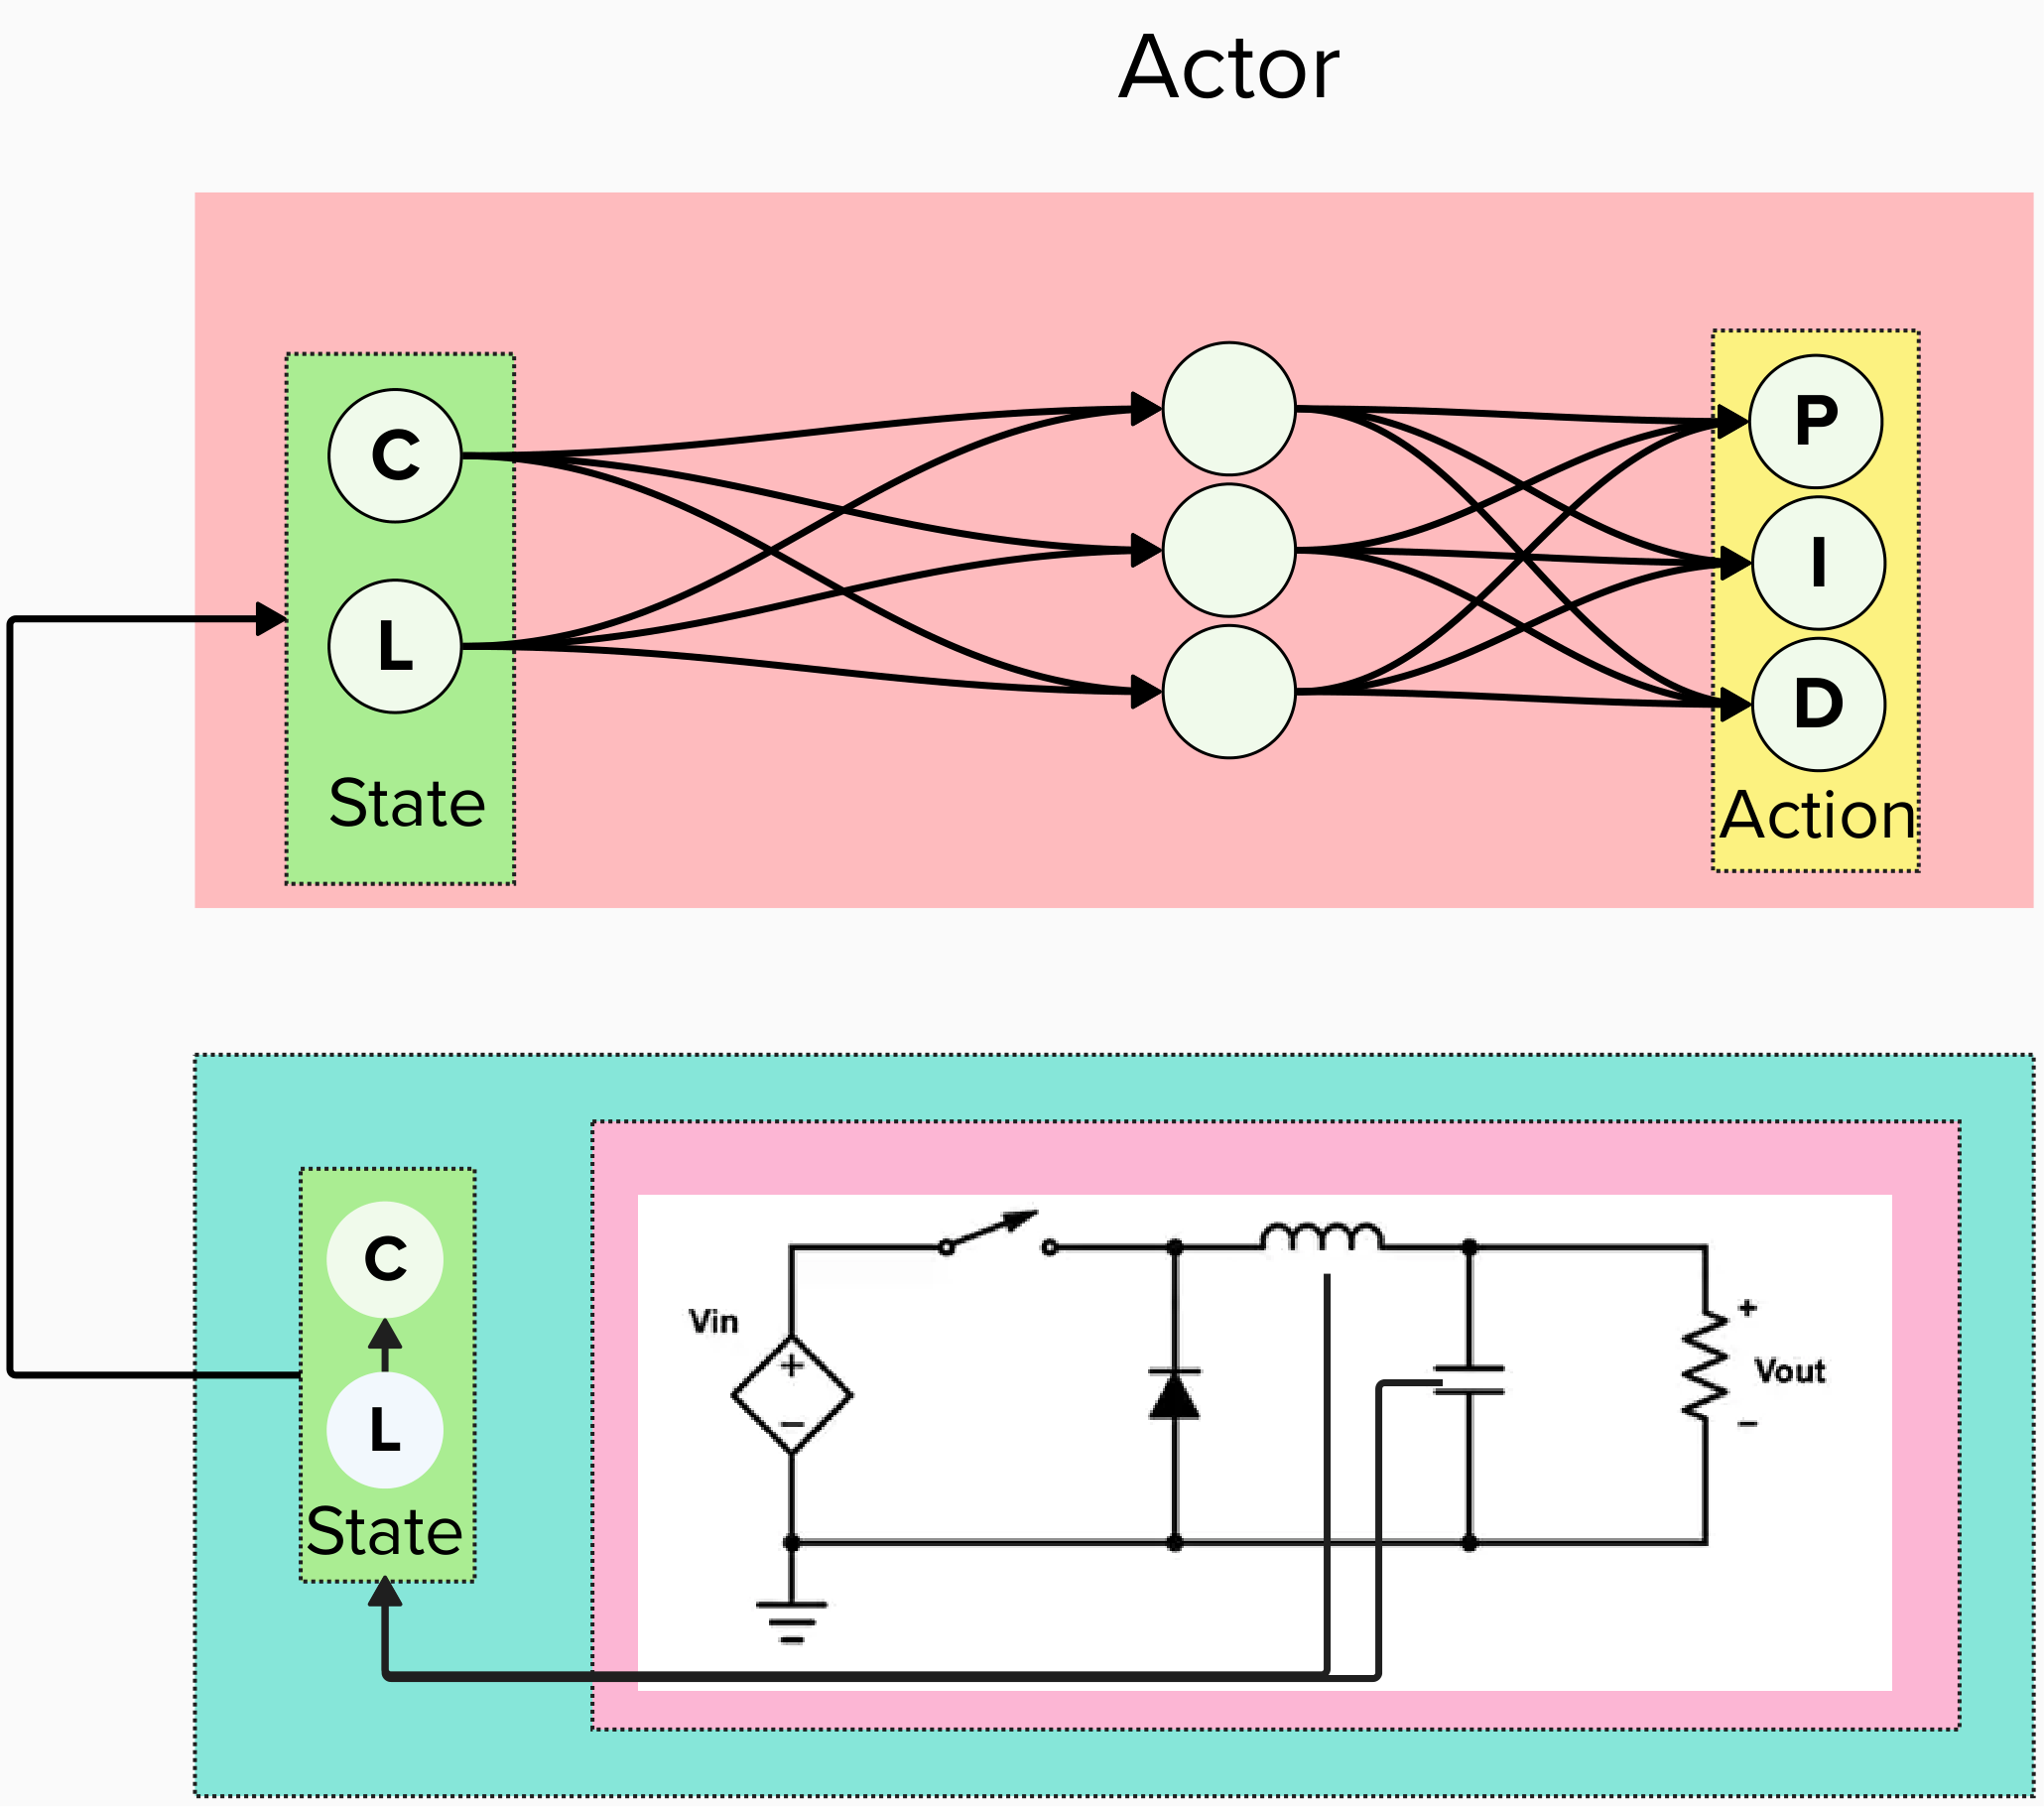
\includegraphics[width=0.5\textwidth]{3Experiment/2Experiment/2Actor.png}
\caption{Die Forward Propagation im Actor-Modul, die den Zustand S (C, L) aufnimmt und über ein mehrschichtiges neuronales Netzwerk PID-Aktionswerte ausgibt.}
\label{fig:actor_decision_making}
\end{figure}


